%%% woptic/doc/woptic_userguide.tex            %%%
%%%                                            %%%
%%% Copyright 2009-2012 Philipp Wissgott       %%%
%%%           2012-2016 Elias Assmann          %%%
%%%

%%% shared-files/header.tex
%%%
%%%    Header for wien2wannier and woptic UGs.
%%%

\documentclass[
   a4paper,
%   oneside,
   twoside,
%   draft
]{wien}
\usepackage[utf8]{inputenc}
\usepackage[osf,sc,slantedGreek]{mathpazo}
\linespread{1.05}
\usepackage[scaled=1.05]{zlmtt}
\usepackage[T1]{fontenc}
\usepackage[protrusion=true,
            expansion=true,
            auto=true,
%            kerning=true,
            spacing=true,
            tracking=false]
           {microtype}

\usepackage{amsmath, amssymb, graphicx, alphabeta, braket, titlepic,
  xspace, minitoc, longtable, siunitx, fancyvrb, enumitem, tabu,
  upgreek, placeins, maybemath}

\usepackage[breaklinks,colorlinks,
            linkcolor=black,
            citecolor=black,
            urlcolor=black,
            ]{hyperref}

\usepackage[textsize=small,colorinlistoftodos]{todonotes}
% TODOs
\newcommand*\tdContent[2][]{\todo[color=orange!30,#1]{#2}}
\newcommand*\tdRef    [2][]{\todo[color=green!30,#1]{#2}}

% \include{texdefine}
\addtolength{\textwidth}{2.5cm}
\addtolength{\oddsidemargin}{-1cm}
\addtolength{\evensidemargin}{-1.6cm}

\newcommand*\name  [1]{\textsc{#1}}
\newcommand*\file  [1]{\texttt{#1}}
\newcommand*\fileit[1]{\texttt{\textit{#1}}}
\newcommand*\code  [1]{\texttt{#1}}
\newcommand*\codeit[1]{\texttt{\textit{#1}}}
% for defaults and the like
\newcommand*\rem   [1]{\textit{\liningnums{#1}}}
\newcommand*\usgrem[1]{\textit{\textrm{#1}}}

\newcommand{\liningnums}[1]{%
  {\fontfamily{pplx}\selectfont #1}}

% lining numbers should go with uppercase
\let\tmp\MakeUppercase
\renewcommand\MakeUppercase[1]{\fontfamily{pplx}\selectfont \tmp{#1}}

\newcommand\MyTOC{
  {
    \linespread{1.1}
    \tableofcontents
  }
}

\newcommand*{\abbrev}[1]{\textsc{#1}}
\newcommand*{\Abbrev}[1]{
  \expandafter\newcommand\csname#1\endcsname{\abbrev{#1}\xspace}
}

\Abbrev{cgs}
\Abbrev{dos}
\Abbrev{soc}
\Abbrev{dft}
\Abbrev{Dft}
\Abbrev{mlwf}
\Abbrev{Mlwf}
\Abbrev{lapw}
\Abbrev{Lapw}
\Abbrev{dmft}
\Abbrev{Dmft}
\Abbrev{uc}
\Abbrev{bz}
\Abbrev{wf}
\newcommand*\wfs{\wf{}s}

\newcommand*\listnote{%
  This file is read using Fortran list-oriented reads, i.e., items are
  separated by white space.%
}

\newcommand\ProgName[2][]{
  \def\myarg{#1}
  \ifx\empty\myarg
     \ProgNameII{#2}{#2}
  \else
     \ProgNameII{#1}{#2}
  \fi
}
\newcommand\ProgNameII[2]{
  \expandafter\newcommand\csname#2\endcsname{%
    \hyperref[sec:#2]{\file{#1}}%
    \xspace%
  }
  \expandafter\newcommand\csname#2Hd\endcsname{%
    \texttt{#1}%
    \xspace%
  }
}

\newcommand\ProgSec[2][]{
  \def\myarg{#1}
  \ifx\empty\myarg
     \def\separator{}
  \else
     \def\separator{---}
  \fi
  \section[\csname#2Hd\endcsname{} \separator{} #1]
  {\csname#2Hd\endcsname{} \separator{} #1}
  \label{sec:#2}
}

\newcommand*\siunits {\abbrev{si}\xspace}

\newcommand*\case    {\texttt{\itshape case}\xspace}
\newcommand*\deffile {\texttt{\itshape def}\xspace}

\newcommand*\wtow   {\href{http://wien2wannier.github.io/}{\textsc{wien2wannier}}\xspace}
\newcommand*\Wtow   {\href{http://wien2wannier.github.io/}{\textsc{Wien2Wannier}}\xspace}
\newcommand*\woptic {\href{http://woptic.github.io/}{\textsc{woptic}}\xspace}
\newcommand*\Woptic {\href{http://woptic.github.io/}{\textsc{Woptic}}\xspace}
\newcommand*\wien   {\href{http://www.wien2k.at}{\textsc{Wien}2k}\xspace}
\newcommand*\Wien   {\href{http://www.wien2k.at}{\textsc{Wien}2k}\xspace}
\newcommand*\wannier{\href{http://www.wannier.org}{\textsc{wannier90}}\xspace}
\newcommand*\Wannier{\href{http://www.wannier.org}{\textsc{Wannier90}}\xspace}
\newcommand*\xcrys  {\href{http://www.xcrysden.org}{XCrySDen}\xspace}
\newcommand*\vesta  {\href{http://jp-minerals.org/vesta/en/}{\textsc{vesta}}\xspace}
\newcommand*\Vesta  {\href{http://jp-minerals.org/vesta/en/}{\textsc{Vesta}}\xspace}
\newcommand*\gnuplot{\href{http://www.gnuplot.info}{gnuplot}\xspace}

\DeclareMathOperator{\tr}{tr}
\DeclareMathOperator{\sgn}{sgn}
\renewcommand*\Re{\mathop{\operatorname{Re}}}

\newcommand*\dd      {\text{d}}
\newcommand*\ii      {\text{i}}
\newcommand*\ee      {\text{e}}

\newcommand{\mb}{\boldsymbol}

%%%% Including template files %%%%
%%%% User code must set \TemplateDir
\newcommand*\FancyVerbStopString{} % empty line ends template inclusion

%%% begin deep magic %%%
\expandafter\def\expandafter\setCatCode\expandafter{
  \catcode35 = 13 % # = active
}
\expandafter\def\expandafter\resetCatCode\expandafter{
  \catcode35 =  6 % # = argument
}
\setCatCode
\def#{\color{gray}\itshape\char35}
\resetCatCode
\newcommand{\Template}[2][]{%
  \\[\baselineskip]
  \begin{minipage}{\linewidth}
    \VerbatimInput[%
    codes={ \setCatCode },
    label={%
      [\raisebox{-.5\height}{\case.#2}]%
      \raisebox{-.5\height}{end of \case.#2}%
    },
    frame=lines, framesep=3mm,
    numbers=left,
    #1
    ]{\TemplateDir/case.#2}
  \end{minipage}
  \\[\baselineskip]
}
%%% end deep magic %%%

\newenvironment{usage}{%
  \list{}{
    \leftmargin    .5\parindent
    \listparindent 0em
    \itemindent    \listparindent
    \linespread{1.1}
  }
  \item\relax\ttfamily%
}{\endlist}

\newlist{options}{description}{1}
\setlist[options]{
  font=\ttfamily, itemsep=0em,
  labelindent=.5\parindent, leftmargin=!, labelsep=1em
}

\newlist{linesI}{enumerate}{1}
\setlist[linesI]{
  font=\bfseries,
  label={line \arabic*}
}

\newenvironment{lines}{%
  \begin{linesI}%
    \newcommand*\T[1]{\texttt{\textit{##1}}}
    \newcommand*\U[1]{\si{##1}}
    \newenvironment{flin}[3][V]{%
      \newcolumntype V {>{\ttfamily}l}
      \newcolumntype T {>{\ttfamily\itshape}l}
      \newcolumntype U {s}
      \def\argIII{##3}
      \ifx\empty\argIII
      \else
        \def\argIII{ --- ##3}
      \fi
      \item \code{##2}\argIII
      \vskip-.5\baselineskip    % longtabu produces an inordinately
                                % large separation
      \begin{longtabu} to \linewidth { V ##1 X}
    }{%
      \end{longtabu}%
    }%
    % \newcommand{\flinbrk}{% — does not work
    %   \endtabu\endgroup
    %   \begingroup\tabu to \linewidth { *2{ >{\ttfamily}l } X}%
    % }%
  }{%
  \end{linesI}%
}

\setcounter{minitocdepth}{1}
\setcounter{secnumdepth}{1}
\setcounter{tocdepth}{1}
\dominitoc


%%% Local Variables: 
%%% mode: latex
%%% End: 

%%% Time-stamp: <2016-04-08 16:32:19 assman@faepop36.tu-graz.ac.at>


\usepackage{mathtools}

\newcommand\TemplateDir{../templates/}

\usepackage{tikz, manfnt, pbox}
\usetikzlibrary{shapes, arrows, chains, decorations.shapes, fit}

\newcommand*\lvir[1][]{%
  \tikz[overlay]
  \node[xshift=-6mm, yshift=-1mm, anchor=base, #1]
  {\footnotesize\textdbend};%
}

\newcommand*\TOCvir{\lvir[xshift=-11.5mm]}

\newcommand*\tocvir[1][]{%
  \tikz[overlay]
  \node[xshift=-3.5em, yshift=-.8mm, anchor=base, #1]
  {\tiny\textdbend};%
}

\newcommand*\rvir[1][]{%
  \tikz[overlay]
  \node[xshift=+6mm, yshift=-1mm, anchor=base, #1]
  {\footnotesize\textdbend};%
}

\newcommand\ProgSecVir[2][]{
  \def\myarg{#1}
  \ifx\empty\myarg
     \def\separator{}
  \else
     \def\separator{---}
  \fi
  \section[\tocvir\csname#2Hd\endcsname{} \separator{} #1]
  {\TOCvir\csname#2Hd\endcsname{} \separator{} #1}
  \label{sec:#2}
}

\ProgName[woptic\_main] {womain}
\ProgName[refine\_tetra]{reftet}
\ProgName[obtain\_dist] {obdist}
\ProgName[woptic]       {woprog}
\ProgName               {kanalysis}
\ProgName               {joinham}
\ProgName[compute\_vr]  {compvr}
\ProgName[convert\_vr]  {convvr}
\ProgName               {wopticlean}
\ProgName               {inwopcheck}

\newcommand*\lapwi   {\file{lapw1}\xspace}
\newcommand*\lapwso  {\file{lapwso}\xspace}
\newcommand*\optic   {\file{optic}\xspace}
\newcommand*\prepwiiw{\file{prepare\_w2wdir}\xspace}
\newcommand*\wiiw    {\file{w2w}\xspace}
\newcommand*\wannierx{\file{wannier90.x}\xspace}
\newcommand*\convham {\file{convham}\xspace}
\newcommand*\wophist {\file{\case.wophist.zip}\xspace}

\newcommand*\td{-{}-}

\newcommand*\hateq{\mathbin{\widehat=}}

\date{for version 1.0.0-$α$}
\author{\name{Elias Assmann} \and \name{Philipp Wissgott}}
\newcommand*\tit{\Woptic User's Guide}
\newcommand*\subtit{Optical conductivity with Wannier functions}
\title{\tit\\[1em]\large\mbox{\it \subtit.}}
\titlepic{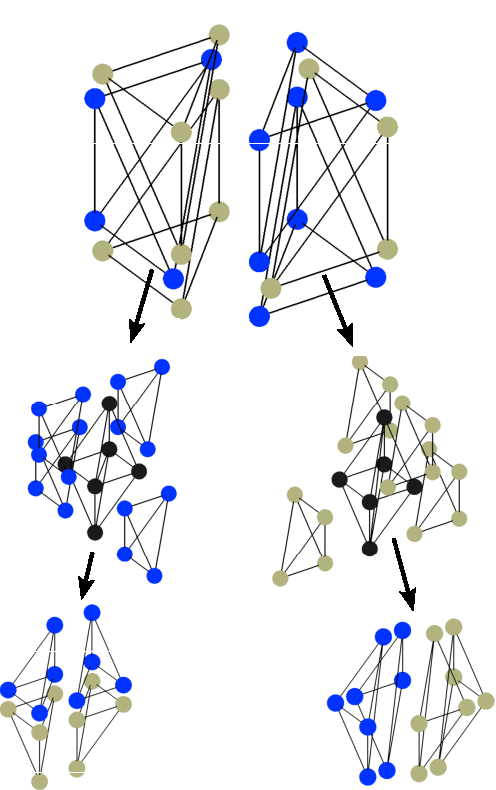
\includegraphics[height=9 cm]{woptic_pic}}

\hypersetup{
  pdftitle={\tit},
  pdfauthor={E. Assmann and P. Wissgott},
  pdfsubject={\subtit},
}
\begin{document}

\raggedbottom

\frontmatter
\maketitle

\newcommand*\cbox[1]{%
  \pbox{\paperwidth}{\relax\ifvmode\centering\fi%
    #1%
  }}

\tikz[overlay, remember picture]
\node[anchor=center] at (current page.center) {
  \begin{minipage}{10.7cm}
    \newcommand*\xL{\color{darkgray}}
    \newcommand*\xW{\color{green!80!black}}
    \newcommand*\xF{\bfseries}
    \newcommand*\xC{\color{brown}}
    \newcommand*\xA{\color{cyan!90!black}}
    \newcommand*\xB{\normalfont\ttfamily}
    \VerbatimInput[commandchars=\!\{\}]{logo.tex}
  \end{minipage}
};

\chapter*{Introduction}
\label{chap:intro}

To compute the optical conductivity $σ$ in the basis of
maximally-localized Wannier orbitals the package \woptic is provided.
It uses the Green function formalism, which yields
%
\begin{equation}
  \label{eq:optcond}
  \tag{$*$}
  σ^{αβ}(Ω) = \tfrac{e^2}{(2π)^2}
  \int\!\dd^3 k \int\!\dd ω\mathop{} \frac{f(ω)-f(ω+Ω)}{Ω}
  \tr\left[A(k,ω)\,V^α(k)\,A(k,ω+Ω)\,V^β(k)\right],
\end{equation}
%
where $σ^{αβ}$ is the $(α,β)$ element of the optical conductivity
tensor ($α,β \in \{x,y,z\}$), $V_\text{uc}$ the unit cell volume, $f$
the Fermi function, $A= \frac\ii{2 π}(G-G^\dagger)$ the generalized
spectral function \cite{Wissgott2012,Tomczak2009a,Jan}, and $V^α$ the
group velocity in direction $α$. The numerical bottleneck in
evaluating \eqref{eq:optcond} is the k-summation, since usually many
k-points are required to obtain converged results. For a speed-up in
k-mesh convergence, \woptic therefore employs an adaptively refined
tetrahedral tiling of k-space.

\Woptic consists of two main programs: \womain, which calculates the
optical conductivity, and \reftet, where the k-mesh is refined; as
well as several smaller support programs.  The individual programs are
normally called by means of the driver script \woprog.  This guide
provides technical documentation for \woptic.  For details on the
underlying formalism and algorithm, see Refs.~\cite{Philipp, Elias,
  woptic}.

\paragraph{Acknowledgement} Development of this software was supported
by Vienna University of Technology, Graz University of Technology, and
the European Research Council through grant agreement no. 306447.

\paragraph{Caution} Following the many recent changes in \wtow and
\woptic, some parts of the older version of \woptic have not yet been
adapted.  As such, they must be considered experimental.  We keep such
untested (or even known to be broken) features in the code and in this
guide, where they are marked with a ``dangerous bend'' sign,
\raisebox{.5\height}{{\footnotesize\dbend}}.

\paragraph{Citation} In any scientific publications arising from the
use of \woptic, we ask that you cite Ref.~\cite{woptic},
%
\begin{quote}
  \href{http://www.sciencedirect.com/science/article/pii/S0010465515004488}{
    \name{E. Assmann, P. Wissgott, J. Kuneš, A. Toschi, P. Blaha}, and
    \name{K. Held},\\
    Comput. Phys. Commun. 202, 1 (2016)
  }
  \href{http://arxiv.org/abs/1507.04881}{arXiv:1507.04881},
\end{quote}
%
to acknowledge your use of our code.  This is in addition to the
appropriate citations to acknowledge other codes used (such as \wien
\cite{wien2k}, \wannier \cite{wien2wannier}, and \wtow
\cite{wannier90}).

\paragraph{Common options and other resources} This guide attempts to
document the features most relevant to the \woptic user; it will not
list every option or every file used by every command.  Most commands
honor the option \code{\td help}, which should provide a definitive
list of options for that command.  The \woptic distribution also
includes a terse instruction sheet as \file{doc/WOPTICHEAT}.

\paragraph{Contributing} \Woptic is Free Software.  You can contribute
to it through \href{https://github.com/woptic/woptic}{GitHub}.  Bug
reports, feature requests, etc. can be submitted there under
\href{https://github.com/woptic/woptic/issues}{Issues}.

\MyTOC

\mainmatter


\chapter{The driver script \woprogHd}
\label{sec:woprog}

\tikzset{
% <on chain> *and* <on grid> reduce the need for manual relative
% positioning of nodes
  >=latex, %shorten >=1pt,
  % somehow, I need ‘on grid, on chain’ both globally and in every
  % node
  flowchart/.style = {
    every node/.style = { on chain, on grid },
    every join/.style={norm},   % Default linetype for connecting boxes
    base/.style={ align=center, draw },
    prog/.style={
      base, rectangle, minimum width=8em, inner sep=2mm,
      execute at begin node=\ttfamily % ‘font=’ screws up align
    },
    file/.style={
      base, ellipse,
      execute at begin node=\ttfamily % ‘font=’ screws up align
    },
    heading/.style={
      base, rounded rectangle, inner sep=10pt,
      outer sep=0pt
    },
    mycloud/.style={
      base, cloud, aspect=2.2, cloud puffs=20, cloud puff arc=135,
      inner sep=0
    },
    test/.style={base, diamond, aspect=2, text width=5em},
    coord/.style={ },
    norm/.style={->},
    old/.style ={dashed, overlay},
  }
}

This is the main user-callable program.  It runs the other programs as
necessary until a set number of iterations is completed (or an error
occurs) --- convergence has to be checked manually.  If you include an
outer window in your \code{interp} calculation, you should check the
localization of $W^{αβ}(R,ω)$ and/or the interpolation errors in the
optical conductivity.

Since the procedure is a little involved, we provide
Fig.~\ref{fig:woptic_iter} to give an overview of the files and
programs involved in one iteration (but note that not all files that
might be involved are shown).  The computation of the group velocities
$V^α(k)$ for the new k-points varies according to the
\hyperref[woprog:matelmode]{option \code{matelmode}}.  \Woptic
implements two modes using the full momentum matrix elements
$V_{ab}^α(k) = \braket{ψ\mathop{} ak | \mathop{\widehat p_α} |
  ψ\mathop{} bk}$ as group velocities:

\paragraph{\code{optic} mode} takes the matrix elements from \wien's
\optic module,
%
\begin{gather*}
  \tikz[flowchart, baseline, start chain]
  \node [mycloud] {get new momentum\\matrix elements};
  \,=\,
  \begin{tikzpicture}[
    flowchart, baseline,
    start chain=going right, node distance=4mm,
    prog/.append style={minimum width=3.8em,text width=, },
    ]
    \node [prog, anchor=base] {\lapwi};
    \node [file, join]        {vector};
    \node [prog, join]        {\optic};
    \node [file, join]        {mommat2};
  \end{tikzpicture}\;,
\end{gather*}
% 
and transforms them to the Wannier basis using the matrices $U(k)$
which diagonalize the Wannier-interpolated Hamiltonian, $U_{nu}(k)
H^\text{w}_{uv}(k) U_{vm}^\dagger(k) = δ_{nm} ε_n(k)$.  But the
diagonalization fixes the eigenvectors only up to a phase, which leads
to a \emph{random-phase problem} in \eqref{eq:optcond} and associated
uncertainties in the optical conductivity.  The problem is absent
whenever the self-energy is orbital-independent (by symmetry, or in a
noninteracting model).  In such a case, \code{optic} mode should be
dependable.  Otherwise, the results should be checked for the
influence of the random-phase problem.

\paragraph{\code{interp} mode} applies Wannier interpolation to the
matrix elements directly in order to overcome the random-phase
problem.  \compvr calculates the Wannier momentum matrix elements in
direct space
%
\begin{gather*}
  V^{\text{w},α}_{uv}(R) = \frac1{N_k} \sum_k \ee^{-\ii k\cdot
    R}\, U_{un}^\dagger(k) V^α_{nm}(k) U_{mv}(k) =
  \braket{w\mathop{} u0 | \mathop{\widehat p_α} | w\mathop{}
    vR},
\end{gather*}
%
and \convvr interpolates them to the new k-points,\footnote{In the
  interest of full disclosure, the diagram is accurate in the case
  where only Wannier-Wannier transitions are taken into account.  With
  mixed transitions, \file{vr} is supplemented by \file{vvr} and
  \file{vk$α$} by \file{vvk$αβ$}, and \optic is also called for the
  mixed [Wannier-Bloch] matrix elements.}
%
\begin{gather*}
  \tikz[flowchart, baseline, start chain]
  \node [mycloud] {get new momentum\\matrix elements};
  \,=\,
  \begin{tikzpicture}[
    flowchart, baseline,
    start chain=going right, node distance=10mm and 4mm,
    ]
    \node [prog, anchor=base] (convert_vr) {\convvr};
    \node [file, join]                     {vk$α$};
    \node [file, above=of convert_vr, join=with convert_vr by <-]
                                           {vr};
  \end{tikzpicture}\;.
\end{gather*}
%
The interpolation works well for the Wannier-Wannier transitions
($V^{\text{W},α}$), but interpolation errors may become large for the
mixed transitions governed by $W^{αβ}(R,ω)$, where
%
\begin{gather*}
  W^{αβ}_{uv}(k, ω) = \sum_i V^α_{ui}(k) A_{ii}(ω) V^β_{iv}(k)
\end{gather*}
%
with the index $i$ running over the non-Wannier states (i.e.~the outer
window) and the matrix elements are transformed into the Wannier basis
on one side only.  Note that the interpolation errors typically only
affect the interband optical conductivity; as long as the low-energy
degrees of freedom are described by the Wannier functions, the static
quantities (dc conductivity and thermopower) should be reliable.

\paragraph{\lvir In addition, \code{Peierls}} mode uses the Peierls
approximation $V(k) \approx \ii\mathop{\nabla_k} H(k)$ instead of the
momentum matrix elements.  It is currently unsupported.

\paragraph{Further reading.} See \cite{Philipp} for the original
description of \woptic in the \code{optic} and \code{Peierls} modes.
See \cite{Elias} for a detailed description of \code{interp} mode and
a numerical comparison to \code{optic} mode including an analysis of
the errors commited in each of them.  Ref.~\cite{Wissgott2012} tests the
Peierls approximation against the full momentum matrix elements.

\paragraph{\lvir Disentanglement} is supported only in \code{interp}
mode in the case where only Wannier-Wannier transitions are included.
This may be useful when the Wannier model is expected to describe all
the salient features of a system, but disentanglement is necessary,
e.g., to remove extraneous states at the band edges.

%% ------------------------------------------------------------------------
%% Flowcharts inspired by:
%% http://www.texample.net/tikz/examples/flexible-flow-chart/

\begin{figure}
  \centering
  \newlength\dx
  \newlength\dy
  \setlength\dx{22mm}
  \setlength\dy{18mm}
\begin{tikzpicture}[
  flowchart,
  start chain=going below,   % General flow is top-to-bottom
  on chain, on grid,
  node distance=\dy and \dx, % Global setup of box spacing
]

%%% Top
\node [coord]                                (top)          {};

% top left
\node [file,  right=40mm of top,  overlay]   (kcontribw)    {kcontribw};
\node [coord, right=of kcontribw, overlay]   ()             {};
\node [coord, overlay]                       (start)        {};

% top right
\node [file,   left=40mm of top, overlay]    (tetra)        {tetra, map, voe};

% top center
\node [prog,  below=of top, join=with tetra, join=with kcontribw]
                                             (refine_tetra) {\reftet};

% top right
\node [coord, below=of tetra, overlay]        ()            {};
\node [file, overlay, join=with refine_tetra] (tetra_new)   {\ldots\_refined};

%%% Center
\node [file,  below=of refine_tetra, join=with refine_tetra] 
                                              (klist_new)   {klist\_add};
\node [coord]                                 (m1)          {};
\node [coord]                                 ()            {};
\node [coord]                                 (m2)          {};

%%% Right branch
\node [mycloud, right=of m1, yshift=-.4\dy, join=with klist_new]
      (get_mommat) {get new momentum\\matrix elements};
\node [file, yshift=-.6\dy, join]
      (mommat)     {mommat2 \textrm{and/or}\\ vk$α$, vvk$αβ$};

%%% Right branch
\node [prog,  left=of m1, join=with klist_new](convham)     {\convham};
\node [file,  left=2\dx of mommat, join]      (hk)          {hk};

\node [file,  left=1.3\dx of hk, overlay]     (hk_old)      {\ldots\_old};

%%% After re-join
\node [prog, below=of m2, join=with mommat, join=with hk, join=with hk_old]
                                              (joinham)     {\joinham};
\node [file, join]                            (hk_new)      {\ldots\_joined};
\node [file,  left=2\dx of hk_new, overlay]   (k1w)      {K1w\\wdoskcontribw};
\node [prog, below=of hk_new, join, join=with hk_new] (woptic_main) {\womain};
\node [file, join]                            (kcontribw_new){kcontribw\_new};
\node [file, left=2\dx of kcontribw_new, overlay, join=with woptic_main]
                                              (k1w_new)     {\ldots\_new};

%%% Bottom
\node [coord, below=of kcontribw_new]         (bottom)      {};
\node [coord, right=of bottom, overlay]       (end)         {};

%%% ‘old’ and ‘new’ files


%%% Arrows not generated by ‘join’
\draw[old]          (hk_new)        edge[->, bend left=15]   (hk_old);
\draw[old]          (k1w_new)       edge[->, bend left]      (k1w);
\draw[old]          (tetra_new)     edge[->, bend left]      (tetra);
\draw[old]          (kcontribw_new) edge[->, out=-90,in=180] (end);
\draw[old]          (kcontribw)     edge[<-, out=  0,in= 90] (start);
\draw[norm,overlay] (kcontribw) edge[bend left=40] (woptic_main.north east);

\end{tikzpicture}

\caption{Flow of control and information in the main \woptic loop:
  programs (rectangles) and selected files (ellipses).  Dashed lines
  indicate a file is taken from the previous iteration.}
\label{fig:woptic_iter}
\end{figure}

\begin{figure}
  \centering
  \setlength\dx{25mm}
  \setlength\dy{17mm}
\begin{tikzpicture}[%
  flowchart,
  start chain=going below,    % general flow is top-to-bottom
  on chain, on grid,
  node distance=\dy and \dx,% global setup of box spacing
  ]

\node [base]                    (wien2k)        {\wien run};
\node [prog, join]              (prepare)       {\prepwiiw, cd};
\node [base, join]              (wien2wannier)  {\wiiw, \wannierx};

\node [coord, yshift=-.5\dy]     (m1)     {};

\node [heading, left =of m1]    (interp) {momentum matrix\\interpolation};
\node [file, join]                       {inop\\MME=ON};
\node [prog, join]                       {\optic};
\node [prog, join]                       {\compvr};
\node [prog, join]              (woptic) {\woprog};

\node [coord, right=of woptic]  (m2)     {};

\node [heading,    right=of m1] (trad)   {momentum matrix\\from \optic};
\node [file, join]                       {inop\\MME=ON};
\node [prog, join, right=of m2]          {\woprog};

\draw (wien2wannier.south) -- (trad);
\draw (wien2wannier.south) -- (interp);
\end{tikzpicture}

\caption{Flow of control and information in \woptic initialization.}
\label{fig:woptic_init}
\end{figure}


\FloatBarrier
\section{Synopsis}
\label{sec:woprog:usage}

\newcommand\Ntot{$N_\text{tot}$\xspace}
\newcommand\NI{\ensuremath{N_\text{i}}\xspace}

\begin{usage}
  \woprog [-i \Ntot] [\td{}restart $I$] [\codeit{more options}]
\end{usage}


\section{Options}

\begin{options}
\item [-i \Ntot] stop after iteration \Ntot{} \rem{(default: 5)}

\item [\td{}restart $I$] restart from \wophist at the beginning of
  iteration $I$ \rem{(default: 1)}

\item [\td{}restore $I$] restore iteration $I$ from \wophist without
  continuing

\item [\td{}theta $Θ$] refinement harshness \rem{($Θ=\mathit0$: uniform
    mesh, $Θ=\mathit1$: most adaptive; default: 0.5)}

\item [\td{}inter] focus refinement on larger $Ω$

\item [\td{}init \NI] initial uniform refinement steps \rem{(default:
 3)} \label{woprog:init}

\item [\lvir\td{}band] compute optical conductivity contributions along
  \file{\case.klist\_band} to be processed by \kanalysis

\item[-p] call the parallelized versions of \lapwi, \lapwso, \optic
  (\woptic itself is not parallelized)
\end{options}
%
The iterations in \code{-i}, \code{\td{}restart}, and
\code{\td{}restore} are ``absolute'' in the sense that iteration $1$
always corresponds to the initial k-mesh.  Thus, \code{\woprog{}
  \td{}restart 3 -i 5} does three iterations: nos. $3$, $4$, and $5$.
Iteration no. $1$ starts with a uniform k-mesh whose density is
determined by \NI.  The starting mesh corresponds to $(2^{\NI+1})^3$
k-points in the full \bz.

Let $T$ be a tetrahedron and $ε(T)$ its associated integration error
estimate.  The precise meaning of the ``harshness'' $Θ\in [0,1]$ is:
$T$ will be refined if
%
\begin{gather}
  \label{eq:theta}
  \tag{\code{\td{}theta}}
  ε(T) \ge Θ \max_{T} ε(T)
\end{gather}
%
(but may also be refined due to other rules) \cite{Philipp, woptic}.
The \code{\td{}inter} option scales the contributions to the error
estimates by the frequency,
%
\begin{gather}
  \label{eq:inter}
  \tag{\code{\td{}inter}}
  ε(T; Ω) \gets Ω\cdot ε(T,Ω),
\end{gather}
%
for the purposes of refinement.


\section{The input file \file{\case.inwop}}
\label{sec:woprog:inwop}

The main input file for \woptic is
%
\Template{inwop}
%
\listnote

\pagebreak
\begin{lines}
  \begin{flin}{mode, matelmode, intrahop}{modes of operation}
    \label{woprog:matelmode}
    mode & OPT   & compute the optical conductivity\\
         & JOINT & compute the joint density of states
                   (noninteracting only)\\
    matelmode & 1 | Peierls & use $\dd H^\text{w}/\dd k$ as momentum matrix
                              elements\\
              & 2 | interp  & Wannier-interpolated momentum matrix elements\\
              & 3 | optic   & matrix elements computed by \wien's \optic\\
              & 4 | Bloch   & for testing (noninteracting only)\\
              & 5 | LDA     & for testing (noninteracting only;
              should be similar to \optic--\code{joint}--\code{kram})\\
    intrahop & \T{logical} & whether to use intra-\uc hopping in
                             \code{Peierls} mode \cite{Tomczak2009a,Jan}
                             (needs \file{\case.intrahop})
  \end{flin}
  \vskip-.9\baselineskip
  \lvir[anchor=center]{}Only \code{mode}s \code{interp} and \code{optic} are
  thoroughly tested; \code{Peierls}, \code{Bloch}, and \code{LDA} must
  be considered experimental.

  \newcommand*\Emax{\ensuremath{Ω_\text{max}}}
  \newcommand*\dE  {$\upDelta Ω$}
  \newcommand*\Ndiv{$N_{ω/Ω}$\xspace}
  \begin{flin}[T]{\Emax, \dE, $δ$, \Ndiv, $ε$}{frequency grids and broadening}
    \Emax & \U{\eV} & maximum external frequency for which $σ(Ω=\Emax)$
                      is computed\\
    \dE   & \U{\eV} & $Ω$ grid spacing\\
    $δ$   & \U{\eV} & broadening parameter for noninteracting bands
                     (where $Σ \gets \ii\delta$)\\
    \Ndiv & int     & internal frequency density (\Ndiv internal
                      $ω$ per external $Ω$)\\
    $ε$   & real    & tolerance for $ω$-integration limits 
                      ($-\Emax \lesssim ω \lesssim 0$)
  \end{flin}
  \vskip-.9\baselineskip
  \textbf{Note:}\hspace{1em} Set $\Emax=0$ to compute only the dc
  quantities.

  \begin{flin}[T]{Wlo, Whi, [Blo, Bhi]}{band windows}
    Wlo, Whi & int & band indices corresponding to \wfs\\
    Blo, Bhi & int & the outer (``Bloch'') window
                     \rem{(optional, default: \code{Wlo, Whi})}
  \end{flin}

  % We do not use column type [U] here because that way the units are
  % centered
  \begin{flin}{$β$, $μ$}{grand-canonical ensemble parameters}
    $β$ & \U{\eV^{-1}} & the inverse temperature \rem{(To convert to
                         temperature in Kelvin: 
                         $T \hateq \maybeit{11604}/β$.)}\\
    $μ$ & \U{\eV}      & the chemical potential \rem{(applied only to 
                         the interacting bands [see \code{iself}],
                         use the DMFT value; for noninteracting calculations,
                         set $μ=\mathit{0}$)}
  \end{flin}

  \begin{flin}[T]{Drudesep, orbresolv}{}
    Drudesep  & \U{\eV} & cutoff for Drude sumrule integration\\
    \lvir
    orbresolv & logical & whether to compute observables per-orbital
                          (currently deactivated)
  \end{flin}

  \begin{flin}[T]{selfE, Nself}{self-energy specification}
    selfE & logical & whether to read self-energy $Σ_i(ω)$ 
                      from \file{\case.selfE}\\
    Nself & int     & number of bands with self-energy, or $0$
                      \rem{(in this case, $\code{Whi}-\code{Wlo}+1$)}
  \end{flin}

  \begin{flin}[T]{iself}{interacting bands \rem{(ignored if
        \code{selfE=.false.} or \code{Nself=0})}}
    iself & int(Nself) &
    indices of interacting bands \rem{(if \code{Nself=0}: inner window)}
  \end{flin}

  \begin{flin}[T]{wfrot, shift, Eshift, Nshift}{\wf rotation and
      scissors operator}
    wfrot  & logical  & whether to apply unitary matrix from 
                        \file{\case.wfrot} to \wf basis\\
    shift  & logical  & whether to apply rigid ``scissors'' shift\\
    Eshift & \U{\eV}  & shift value\\
    Nshift & int      & number of bands to shift\\
  \end{flin}

  \begin{flin}[T]{ishift}{scissor bands}
    ishift & int(Nshift) & indices of bands to shift
  \end{flin}
\end{lines}


\section{Environment variable \code{\$SCRATCH}}
\label{sec:woprog:scratch}

\woprog and the programs it calls support \wien-style \code{\$SCRATCH}
for temporary files.  This means that \lapwi and \optic will place
\file{\case.vector} and \file{\case.mommat2} in the directory
\code{\$SCRATCH}; likewise, \womain and \reftet will place certain
temporary files in that directory.

However, note that a true local \code{\$SCRATCH} on a cluster is not
supported.  In this case, the individual
\file{\case.mommat2\_\textit{i}} would have to be transferred to the
“master” node.


\section{Output files}
\label{sec:woprog:output}

Over the course of the iterations, \woprog writes diagnostic
information to standard output and lists the executed commands in
\file{:log}.  In particular, the current values of the quantities
\code{thermopower}, \code{dc conductivity}, and \code{sumrules} are
extracted from \womain's output file \file{\case.outputwop}, as well
as the integration error \code{estimator} from \reftet's
\file{case.outputref}.  The latter is given in arbitrary units and
should decrease over the iterations.

The optical conductivity is written to \file{\case.optcondw}.  For
comparison with \wien's standard \optic module, note that there is a
factor $\approx 1112.65$ between \optic's output (given in Gaussian
\cgs units of \SI{e15}{\per\second} in \file{\case.sigmak}) and
\woptic's (in \siunits units of \si{\siemens\per\cm}).  Expressed in
the \siunits, the conversion is $\text\optic = \text\woptic \cdot 4π\,
ε_0\, \SI{e15}{\hertz\ohm\cm}$.

The density of states is written to \file{\case.wdos}.  The files
\file{\case.optcondw} and \file{\case.wdos} always correspond to the
latest iteration.  Together with certain other files, they are
archived in \wophist with a suffix \file{.$I$} for iteration $I$.


\chapter{Support Programs}
\label{sec:support}

In this section, the sub-programs called by \woprog are documented,
roughly in order of decreasing user-callability.


%%%%%%%%
\ProgSec[remove left-over files from \woptic runs]{wopticlean}
%%%%

\wopticlean preserves files which serve as input to \woprog and its
sub-programs, as well as the archive file \wophist.  The number of
files considered for deletion is substantial; to check which ones are,
use the \code{\td recon} option or the source.

\subsection{Synopsis}

\begin{usage}
  \wopticlean [\td recursive] [\td mrproper] [\td recon]
              [\codeit{directory} \ldots]
\end{usage}

\subsection{Options and arguments}

\begin{options}
\item [-r|\td recursive] Operate recursively on \emph{all} directories
  below
\item [-A|\td mrproper] delete also files whose basename does not
  match the containing directory
\item [-n|\td recon] dry-run; print file names that would be deleted
\end{options}
%
The arguments specify \codeit{directories} to operate on
\rem{(default: \file{.})}.  Before a big cleanup (especially when
using \code{-A} or \code{-r}), you are advised to do a dry-run.


%%%%%%%%
\ProgSec[compute $\maybebmsf{V^\text{w}(R)}$]{compvr}
%%%%

\compvr computes the dipole matrix elements $V^{\text{W},α}(R)$ and
$W^{αβ}(R, ω)$ in direct space by applying the matrices $U(k)$ and a
Fourier transform for use with the \code{interp} mode.  You should
check these matrix elements (especially $W^{αβ}$) for decay in $R$
when using this mode.

\subsection{Synopsis}
\begin{usage}
  \compvr [\td text] \case
\end{usage}

\subsection{Option}
\begin{options}
\item [\td text] output \file{\case.vvr} in plain text
\end{options}

\subsection{Files read}
\begin{options}
\item[\case.inwop] input file
\item[\case.chk] \wannier checkpoint file
\item[\case{}\_hr.dat] Hamiltonian in direct space
\item[\case.mommat2] momentum matrix elements
\item[\case.struct] \wien master input file \usgrem{(mixed
    transitions)}
\item[\case.energy] energies from \lapwi \usgrem{(mixed transitions)}
\item[\case.fermi] Fermi energy \usgrem{(mixed transitions)}
\item[\case.inwf] \wiiw input file \usgrem{(disentanglement)}
\end{options}

\subsection{Files written}
\begin{options}
\item[\case.outputvr] log file
\item[\case.vr] $V^{\text{W},α}(R)$
\item[\case.vvr] $W^{αβ}(R, ω)$ \usgrem{(mixed
    transitions)}
\end{options}


%%%%%%%%
\ProgSecVir[$\maybebmsf{σ(k,ω)}$ on a BZ path]{kanalysis}
%%%%

This program generates files that can be used for analysis of the
contributions to the optical conductivity in \woptic.  Required is a
run of \woprog with the \code{\td{}band} option, such that it computes the
contributions to the optical conductivity along
\file{\case.klist\_band} and stores them in
\file{\case.kcontribw\_band}.  \kanalysis reads this file and
generates 2\textsc{d} data in $ω$- and k-space readable e.g. by
gnuplot.

\subsection{Synopsis}
\newcommand*\Nfreq{$n_{Ω}^\text{min}$\xspace}
\begin{usage}
  \kanalysis \Nfreq \case [\codeit{mode}]
\end{usage}

\subsection{Arguments}
\begin{options}
\item [\Nfreq] minimum frequency index for output

\item [\codeit{mode}] \rem{(optional)} by default, the output includes
  extra newlines for convenient plotting with \gnuplot (\code{splot
    "\case.optanalysis\_band" with pm3d}); if $\code{mode} = 1$,
  these newlines are omitted
  
\end{options}


%%%%%%%%
\ProgSecVir[intra-UC hopping for \code{Peierls}]{obdist}
%%%%

In \woptic, for the generalized \code{Peierls} approximation
\cite{Tomczak2009a}, the distances between the Wannier centers are
required.  This program reads \file{\case{}\_centres.xyz} which is
produced by \wannier and generates \file{\case.intrahop} which can
then be used by \woptic.

\subsection{Synopsis}
\begin{usage}
  \obdist \case
\end{usage}


%%%%%%%%
\ProgSec[parse \file{inwop} file]{inwopcheck}
%%%%

A helper program for \woprog.  Reads an \file{inwop} file and outputs
information suitable for reading in a shell script or for inspection.

\subsection{Synopsis}
\begin{usage}
  \inwopcheck \case.inwop
\end{usage}


%%%%%%%%
\ProgSec[k-integration]{womain}
%%%%

\womain computes the optical conductivity contributions $σ(k,ω)$ on
the k-mesh constructed by \reftet and performs the k- and
$ω$-integration.  It is normally called by \woprog, but it may be
useful to call it manually after a \woprog run.

\subsection{Synopsis}
\begin{usage}
  \womain [\td{}band] \case
\end{usage}

\subsection{Option}
\begin{options}
\item [{\lvir[xshift=-2.65mm]}\td{}band] compute optical conductivity
  contributions along \file{\case.klist\_band} to be processed by
  \kanalysis
\end{options}

\paragraph{} Files used by \womain are listed below.  \emph{Updated}
files are written with a suffix \file{\_new}.  Which files precisely
are used depends on the options in effect, this dependence is
partially indicated below.

\subsection{Files read}
\begin{options}
\item [\case.inwop] woptic main input file \usgrem{(always)}
\item [\case.struct] Wien2k master input file \usgrem{(always)}
\item [\case.symop] symmetry operations from optic \usgrem{(always)}
\item [\case.klist] symmetrized k-points \usgrem{(always)}
\item [\case.tetra] symmetrized tetrahedra \usgrem{(always)}
\item [\case.energy] energies from \lapwi
\item [\case.fermi] Fermi energy
\item [\case.mommat2] matrix elements from \optic
\item [\case.chk] \wannier checkpoint file \usgrem{(testing mode)}
\item [\case.vk$α$] Wannier-interpolated matrix elements
  \codeit{(interp)}
\item [\case.vvk$αβ$] Wannier-interpolated mixed matrix elements
  \codeit{(interp)}
\item [\case.hk] Wannier Hamiltonian $H^\text{w}(R)$
\item [\case.selfE] self-energy $Σ(ω)$ \codeit{(selfE)}
\item [\case.wfrot] Wannier function rotation matrix \codeit{(wfrot)}
\item [\case.klist\_full] unsymmetrized k-points
  \codeit{(Peierls)}
\item [\case.tetra\_full] unsymmetrized tetrahedra \codeit{(Peierls)}
\item [\case.map] mapping of \file{klist\_full} to \file{klist}
  \codeit{(Peierls)}
\item [\case.intrahop] \wf center distance matrix \codeit{(Peierls \&
    intrahop)}
\end{options}

\subsection{Files written}
\begin{options}
\item[\case.outputwop] diagnostic output \usgrem{(always)}
\item[\case.optcondw] optical conductivity \usgrem{(always)}
\item[\case.wdos] (joint) density of states \usgrem{(always)}
\item[\lvir \case.optcondw\_orb$αβ$] orbitally resolved optical
  conductivity \codeit{(orbresolv)} (currently deactivated)
\end{options}

\subsection{Files updated}
\begin{options}
\item[\case.kcontribw] optical conductivity contributions
\item[\case.K1w] thermopower contributions
\item[\case.wdoskcontribw] \dos contributions
\end{options}


%%%%%%%%
\ProgSec[k-mesh refinement]{reftet}
%%%%

\reftet uses the optical conductivity contributions $σ(k, ω)$ to
compute integration error estimates and refine the k-mesh.  It is
normally called by \woprog.

\subsection{Synopsis}
\begin{usage}
  \reftet [\codeit{options}] \case
\end{usage}

\subsection{Options}
\begin{options}
\item[\td theta $Θ$] $0 \le Θ \le 1$ defines the ``harshness'' of
  refinement \usgrem{(see \hyperref[eq:theta]{corresponding option} of
    \woprog)}
\item[\td init \NI] initial refinement with \NI steps \usgrem{(see
    \hyperref[woprog:init]{corresponding option} of \woprog)}
\item[\td inter] give larger weight to higher-energy contributions
  \usgrem{(see \hyperref[eq:inter]{corresponding option} of \woprog)}
\end{options}

\paragraph{} Files used by \reftet are listed below.  \emph{Updated}
files are written with a suffix \file{\_refined}.

\subsection{Files read}
\begin{options}
\item[\case.inwop] woptic main input file
\item[\case.struct] Wien2k master input file
\end{options}

\subsection{Files written}
\begin{options}
\item[\case.kcontribw] function values for estimator on
  \file{\case.klist}
\item[\case.outputref] log file
\end{options}

\subsection{Files updated}
\begin{options}
\item[\case.klist] symmetrized k-points
\item[\case.klist\_full] unsymmetrized k-points
\item[\case.tetra] symmetrized tetrahedra
\item[\case.tetra\_full] unsymmetrized tetrahedra
\item[\case.voe] list of k-points on tetrahedral edges
\item[\case.map] internal mapping of \file{\case.klist\_full} to
  \file{\case.klist}
\end{options}


%%%%%%%%
\ProgSec[combine \file{hk} / \file{mommat2} / \file{vk$α$} /
\file{vvk$αβ$} files]{joinham}
%%%%

\joinham combines \file{\_old} files from the previous iteration with
new files corresponding to added k-points.  It is normally called by
\woprog.

\subsection{Synopsis}
\begin{usage}
  joinham \case                                      |\\
  joinham \codeit{hk}   \codeit{mommat}              |\\
  joinham \codeit{hk1}  \codeit{hk2}  \codeit{hkout} |\\
  joinham \codeit{hk1}  \codeit{hk2}  \codeit{hkout} 
          \codeit{mom1} \codeit{mom2} \codeit{momout}
\end{usage}

\subsection{Arguments}
\begin{options}
\item [\itshape hk*] a file of type \file{\case.hk},
  \file{\case.vk$α$}, or \file{\case.vvk$αβ$}
\item [\itshape mom*] a file of type \file{\case.mommat2}
\end{options}
%
In the first form, \file{\case.hk\_old} is joined with
\file{\case.hk}, and, if they exist, \file{\case.mommat2\_old} with
\file{\case.mommat}.  In the second form, \file{\codeit{hk}\_old} is
joined with \fileit{hk} and \fileit{mom\_old} with \fileit{mom}.  In
both cases, output file names are suffixed with \file{\_joined}.
\code{Unformatted} \fileit{mom} files are handled automatically and
result in \code{unformatted} output.


%%%%%%%%
\ProgSec[Fourier-interpolate $\maybebmsf{V^\text{w}(k)}$]{convvr}
%%%%

\convvr computes \file{\case.vk$α$} and \file{\case.vvk$αβ$} from
\file{\case.vr} and \file{\case.vvr} by Fourier transform.  The
procedure is analogous to \file{convham}, \file{\case.hk}, and
\file{\case{}\_hr.dat}.

\subsection{Synopsis}
\begin{usage}
  \convvr [\td text] \case
\end{usage}

\subsection{Option}
\begin{options}
\item [-t, \td text] write \file{\case.vvk$αβ$} in plain text instead
  of \code{unformatted} (\file{\case.vk$α$} is always plain text)
\end{options}

\subsection{Files read}
\begin{options}
\item[\case.struct] \wien master input file
\item[\case.klist] target k-points
\item[\case.inwop] \woprog input file
\item[\case.vr] direct-space matrix elements $V^{\text{W},α}(R)$
\item[\case.vvr] direct-space mixed matrix elements $W^{αβ}(R, ω)$
  \rem{(mixed transitions)}
\end{options}

\subsection{Files written}
\begin{options}
\item[\case.outputvk] log file
\item[\case.vk\{x,y,z\}] k-space matrix elements $V^{\text{W},α}(k)$
\item[\case.vvk\{xx,xy,xz,yy,yz,zz\}] k-space mixed matrix elements
  $W^{αβ}(R, ω)$ \rem{(mixed transitions)}
\end{options}


\backmatter
\begin{thebibliography}{88}
\bibitem{Wissgott2012}
  \name{P. Wissgott, J. Kuneš, A. Toschi,} and \name{K. Held.}
  \textit{Dipole matrix element approach versus Peierls approximation
    for optical conductivity.}
  \href{http://prb.aps.org/abstract/PRB/v85/i20/e205133}{
    Phys. Rev. B {\bf 85}, 205133 (2012).
  }

\bibitem{Tomczak2009a}
  \name{J.M. Tomczak} and \name{S. Biermann.}
  \textit{Optical properties of correlated materials: Generalized
    Peierls approach and its application to $\text{VO}_{2}$.}
  \href{http://prb.aps.org/abstract/PRB/v80/i8/e085117}{
    Phys. Rev. B {\bf 80}, 085117 (2009).
  }

\bibitem{Jan}
  \name{J.M. Tomczak.}
  \textit{Spectral and optical properties of correlated materials.}
  \href{https://pastel.archives-ouvertes.fr/pastel-00003163}{
    PhD Thesis, \'Ecole Polytechnique, Paris (2007).
  }

\bibitem{Philipp}
  \name{P. Wissgott.}
  \textit{Transport properties of correlated materials from first
    principles.}
  \href{http://katalog.ub.tuwien.ac.at/AC07812647}{
    PhD Thesis, TU Wien, Vienna (2012).
  }

\bibitem{Elias}
  \name{E. Assmann.}
  \textit{Spectral properties of strongly correlated materials.}
  \href{http://katalog.ub.tuwien.ac.at/AC12656725}{
    PhD Thesis, TU Wien, Vienna (2015).
  }

\bibitem{woptic}
  \name{E. Assmann, P. Wissgott, J. Kuneš, A. Toschi, P. Blaha,} and
  \name{K. Held.}
  \textit{woptic: optical conductivity with Wannier functions and adaptive
    k-mesh refinement.}
  \href{http://www.sciencedirect.com/science/article/pii/S0010465515004488}{
    Comput. Phys. Commun. \textbf{202}, 1 (2016),
  }
  \href{http://arxiv.org/abs/1507.04881}{arXiv:1507.04881}.

\bibitem{wien2k}
  \name{P. Blaha, K. Schwarz, G.K.H. Madsen, D. Kvasnicka,} and
  \name{J. Luitz.}
  \textit{Wien2k, An Augmented Plane Wave + Local Orbitals Program for
    Calculating Crystal Properties.}
  Techn. Universität Wien, Vienna, (2001).
  \url{http://www.wien2k.at}.

\bibitem{wien2wannier}
  \name{J. Kuneš, R. Arita, P. Wissgott, A.Toschi, H. Ikeda,}
  and \name{K. Held.}
  \textit{Wien2wannier: From linearized augmented plane waves to maximally
    localized Wannier functions.}
  \href{http://www.sciencedirect.com/science/article/pii/S0010465510002948}{
    Comput. Phys. Commun. \textbf{181}, 1888~(2010),
  }
  \href{http://arxiv.org/abs/1004.3934}{arXiv:1004.3934}.

\bibitem{wannier90}
  \name{A.A. Mostofi, J.R. Yates, Y.-S. Lee, I. Souza, D. Vanderbilt,}
  and \name{N. Marzari.}
  \textit{Wannier90: A tool for obtaining maximally-localized Wannier
    functions.}
  \href{http://www.sciencedirect.com/science/article/pii/S0010465507004936}{%
    Comput. Phys. Commun. \textbf{178}, 685~(2008).
  }
  \href{http://arxiv.org/abs/0708.0650}{arXiv:0708.0650}

% Must have empty line to terminate bibitem!

\end{thebibliography}
\end{document}
